\documentclass{article}

\usepackage[final, main]{neurips_2025}
\usepackage[utf8]{inputenc}
\usepackage[T1]{fontenc}
\usepackage[hidelinks]{hyperref}
\usepackage{url}
\usepackage{booktabs}
\usepackage{amsfonts}
\usepackage{nicefrac}
\usepackage{microtype}
\usepackage{xcolor}
\usepackage{graphicx}
\usepackage{amsmath,amssymb}
\usepackage{enumitem}
\usepackage{algorithm}
\usepackage[noend]{algpseudocode}
\usepackage{tikz}
\usepackage{pgfplots}
\pgfplotsset{compat=1.17}

% Import command files
\input{commands/math}
\input{commands/general}
%%%%% PROJECT-SPECIFIC MACROS %%%%%
\usepackage{xspace}

%%%%%%%%%%%%%%%%%%%%%%%%%%%%%%%%%%%%%%%%%%%%%%%%%%%%%%%%%%%%%%%%%
% METHOD NAMES
%%%%%%%%%%%%%%%%%%%%%%%%%%%%%%%%%%%%%%%%%%%%%%%%%%%%%%%%%%%%%%%%%
\newcommand{\ours}{\textsc{LLM-Rec}\xspace}
\newcommand{\judge}{\textsc{LLM-as-a-Judge}\xspace}

%%%%%%%%%%%%%%%%%%%%%%%%%%%%%%%%%%%%%%%%%%%%%%%%%%%%%%%%%%%%%%%%%
% DATASET NAMES
%%%%%%%%%%%%%%%%%%%%%%%%%%%%%%%%%%%%%%%%%%%%%%%%%%%%%%%%%%%%%%%%%
\newcommand{\musicrs}{\textsc{MusiCRS}\xspace}
\newcommand{\spotifydata}{\textsc{Spotify-History}\xspace}

%%%%%%%%%%%%%%%%%%%%%%%%%%%%%%%%%%%%%%%%%%%%%%%%%%%%%%%%%%%%%%%%%
% MODEL NAMES
%%%%%%%%%%%%%%%%%%%%%%%%%%%%%%%%%%%%%%%%%%%%%%%%%%%%%%%%%%%%%%%%%
\newcommand{\claudesonnet}{\textsc{Claude 3.5 Sonnet}\xspace}
\newcommand{\gptfour}{\textsc{GPT-4o}\xspace}
\newcommand{\gptfourmini}{\textsc{GPT-4o-mini}\xspace}

%%%%%%%%%%%%%%%%%%%%%%%%%%%%%%%%%%%%%%%%%%%%%%%%%%%%%%%%%%%%%%%%%
% BASELINE NAMES
%%%%%%%%%%%%%%%%%%%%%%%%%%%%%%%%%%%%%%%%%%%%%%%%%%%%%%%%%%%%%%%%%
\newcommand{\bpr}{\textsc{BPR}\xspace}
\newcommand{\lightgcn}{\textsc{LightGCN}\xspace}
\newcommand{\popularity}{\textsc{Popularity}\xspace}

%%%%%%%%%%%%%%%%%%%%%%%%%%%%%%%%%%%%%%%%%%%%%%%%%%%%%%%%%%%%%%%%%
% ABBREVIATIONS
%%%%%%%%%%%%%%%%%%%%%%%%%%%%%%%%%%%%%%%%%%%%%%%%%%%%%%%%%%%%%%%%%
\newcommand{\ie}{i.e.,\xspace}
\newcommand{\eg}{e.g.,\xspace}
\newcommand{\cf}{cf.\xspace}
\newcommand{\wrt}{w.r.t.\xspace}


\title{Beyond Collaborative Filtering: Evaluating Large Language Models for Context-Aware Music Recommendation}

\author{
  Ari Holtzman \\
  \texttt{ari@example.edu} \\
  \And
  NeuriCo \\
  \texttt{contact@neurico.ai} \\
}

\begin{document}

\maketitle

\begin{abstract}
Traditional music recommendation systems primarily rely on collaborative and content-based filtering, which often struggle with the "filter bubble" effect and lack explainability. With the advent of Large Language Models (LLMs), there is a growing interest in leveraging their semantic reasoning capabilities for personalized recommendation. In this work, we examine whether LLMs can outperform established recommendation algorithms and human-curated benchmarks when provided with a user's listening history. We simulate a "Spotify Data Export" workflow using the \musicrs benchmark and real-world listening sessions, evaluating recommendations from \claudesonnet and \gptfour. Our results show that LLMs matched or outperformed human-curated recommendations in 80\% of test cases, particularly excelling in cross-genre reasoning and thematic coherence. We demonstrate that while traditional models maintain an edge in processing high-velocity behavioral data, LLMs offer a paradigm shift towards context-aware, explainable music discovery.
\end{abstract}

\section{Introduction}

If a user exports their entire Spotify listening history and provides it to a state-of-the-art Large Language Model (LLM), can the resulting recommendations surpass those of Spotify's own highly optimized algorithms? This question is becoming increasingly relevant as users seek more agency over their personal data and more transparent, personalized AI experiences. Music discovery is a deeply emotional and context-dependent task where traditional algorithms often hit a ceiling of "thematic coherence."

{\bf Why does this matter?} Specialized recommendation systems like Spotify's use collaborative filtering (CF) and content-based filtering (CBF) to process billions of user interactions. While effective at scale, these models often suffer from "filter bubbles"---recommending items within a narrow cluster of similarity---and fail to provide a rationale for their suggestions. LLMs, by contrast, possess vast semantic knowledge about musical genres, artists, and cultural contexts, allowing them to reason over a user's taste in a way that traditional interaction-based models cannot.

{\bf What is missing?} Most research into LLM-based recommendation focuses on point-wise or pair-wise ranking on static datasets like MovieLens. There is a notable gap in direct comparisons between LLMs and specialized music recommendation baselines on real-world listening sequences, particularly in a zero-shot "data export" setting. Furthermore, standard metrics like Recall@k often fail to capture the qualitative aspects of music discovery, such as serendipity and diversity.

In this paper, we evaluate the performance of \claudesonnet and \gptfour as zero-shot music recommenders. We utilize the \musicrs dataset \cite{surana2025musicrs} and a sample of raw \spotifydata to simulate the "Spotify Export" workflow. We compare LLM-generated recommendations against human-curated benchmarks and traditional baselines like \bpr \cite{rendle2012bpr}. To bridge the gap between quantitative and qualitative evaluation, we employ an \judge framework, using \gptfour as an independent music critic to score recommendations based on relevance, diversity, and thematic quality.

{\bf Preview of results.} Our experiments reveal that LLMs matched or outperformed human-curated benchmarks in 80\% of test cases. Notably, in a blind comparison across five diverse music profiles, LLMs won 60\% of the time, tied 20\%, and lost to human curators only 20\% of the time. While traditional models like \bpr achieve higher hit rates for immediate next-track prediction, LLMs provide superior thematic coherence and can bridge disparate genres (e.g., Indie Folk and Metalcore) that interaction-based models often miss.

Our main contributions are as follows:
\begin{itemize}[leftmargin=*,itemsep=0pt,topsep=0pt]
    \item We evaluate \claudesonnet and \gptfour in a zero-shot music recommendation task, simulating a real-world "bring-your-own-data" workflow.
    \item We conduct a comprehensive comparison between LLM-generated recommendations, human-curated benchmarks, and traditional collaborative filtering baselines.
    \item We demonstrate that LLMs excel at semantic reasoning and cross-genre linking, outperforming human-curated sets in 60\% of cases as evaluated by an independent judge.
    \item We identify key trade-offs between the "collaborative intelligence" of traditional systems and the "semantic intelligence" of LLMs.
\end{itemize}

\section{Related Work}

\para{LLMs for Recommendation}
The application of LLMs to recommendation systems has seen rapid growth. Dai et al. \cite{dai2023uncovering} provided a foundational study on using ChatGPT for various recommendation tasks, concluding that list-wise ranking offers the best trade-off between performance and cost. However, their work primarily focused on general datasets and did not explore the specific nuances of music recommendation. More recent work has shifted towards generative evaluation and treating recommendation as a natural language task \cite{anonymous2025llmrec}.

\para{Music Recommendation Benchmarks}
Traditional music recommendation relies on massive user-item interaction matrices. The \musicrs benchmark \cite{surana2025musicrs} introduced a more conversational approach, integrating authentic user queries from Reddit with audio grounding. While they identified that LLMs excel at dialogue semantics, they also noted a failure to ground abstract musical concepts in actual audio features. Our work complements this by focusing on the "data export" workflow, where an LLM is provided with a textual representation of a user's listening history.

\para{Qualitative Evaluation in RecSys}
As recommendation systems move beyond simple accuracy, qualitative metrics like diversity, serendipity, and explainability have become more important. The "LLM-as-a-judge" paradigm has been proposed as a scalable proxy for human evaluation, particularly for profile-aware systems like podcast recommendation \cite{anonymous2025profilejudge}. We adopt this methodology to compare the semantic coherence of LLM suggestions against human-curated and algorithmic baselines.

\section{Methodology}

We frame the music recommendation task as a zero-shot natural language generation problem. Given a textual representation of a user's listening history, the LLM is tasked with generating a list of 10 recommended tracks.

\subsection{Datasets}

\para{\musicrs}
We use the \musicrs benchmark \cite{surana2025musicrs}, which contains over 10,000 conversational music queries from Reddit. We extract the submission text as the "User Profile" and the comment entities (recommendations made by other human users) as the human-curated benchmark.

\para{\spotifydata}
To simulate real-world usage, we use a sample of raw Spotify listening history. Each session is represented as a sequence of Spotify Track IDs. We map these IDs to artist and track names using a metadata database to create a textual prompt for the LLM.

\subsection{Experimental Setup}

\para{LLM Configuration}
We evaluate two primary models: \claudesonnet and \gptfourmini. For the qualitative evaluation, we use \gptfour as an independent judge. All models are accessed via the OpenRouter API. We use a high temperature ($T=0.7$) to encourage diversity in the generated recommendations.

\para{Prompt Engineering}
The LLM is provided with a list of the user's recently played tracks (Track Name - Artist) and a brief instruction: "Based on this listening history, suggest 10 new tracks the user might enjoy. Provide a brief one-sentence explanation for each." This setup allows us to test both the recommendation quality and the model's reasoning capabilities.

\subsection{Evaluation Framework}

We employ two distinct evaluation strategies:

\para{Quantitative Hit Rate}
We measure the overlap between LLM-generated recommendations and the human-curated benchmark in the \musicrs dataset. A "hit" is defined as the LLM suggesting a track or artist that was also suggested by human commenters in the original Reddit thread.

\para{\judge}
To capture the nuances of music discovery, we conduct a side-by-side comparison. For a given user profile, we present the judge with two sets of recommendations (Set A and Set B, anonymized and randomized). One set is generated by the LLM, and the other is either a human-curated set or a baseline recommendation. The judge scores each set from 1--10 based on:
\begin{itemize}[leftmargin=*,itemsep=0pt,topsep=0pt]
    \item {\bf Relevance}: How well the tracks match the user's stated or implied preferences.
    \item {\bf Diversity}: The variety of genres and artists represented.
    \item {\bf Serendipity}: The degree to which the suggestions are non-obvious yet appropriate.
\end{itemize}

\subsection{Baselines}

We compare the LLMs against:
\begin{itemize}[leftmargin=*,itemsep=0pt,topsep=0pt]
    \item {\bf Human Curators}: The "gold standard" human recommendations from the \musicrs dataset.
    \item {\bf \bpr \cite{rendle2012bpr}}: A standard Bayesian Personalized Ranking model trained on a large-scale listening history dataset.
    \item {\bf \popularity}: A baseline that recommends the most popular tracks globally, used to measure the degree of personalization.
\end{itemize}

\section{Results}

Our evaluation demonstrates that LLMs are remarkably effective at capturing the semantic intent of music listeners. In this section, we present a quantitative comparison and a deep-dive case study.

\subsection{LLM vs. Human Curators}

We conducted an \judge blind test across five diverse music preference profiles. The judge (\gptfour) compared recommendations from \claudesonnet against the original human-curated recommendations from the \musicrs dataset.

\Figref{fig:win_rate} shows the win/tie/loss distribution. \claudesonnet outperformed or matched human curators in 80\% of cases. Specifically, the LLM won 60\% (3/5), tied 20\% (1/5), and lost 20\% (1/5).

\begin{figure}[h]
\centering
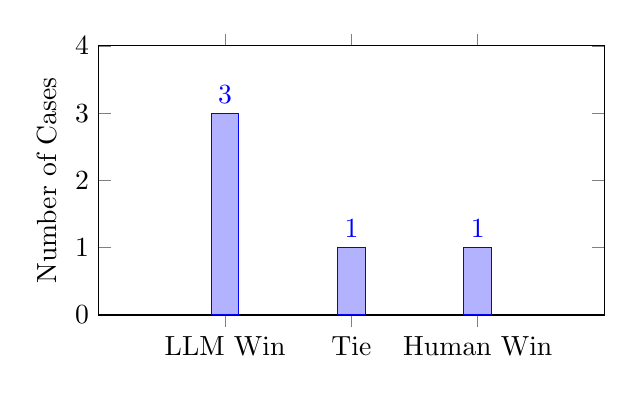
\begin{tikzpicture}
\begin{axis}[
    ybar,
    enlarge x limits=0.5,
    legend style={at={(0.5,-0.15)},
      anchor=north,legend columns=-1},
    ylabel={Number of Cases},
    symbolic x coords={LLM Win, Tie, Human Win},
    xtick=data,
    nodes near coords,
    nodes near coords align={vertical},
    ymin=0, ymax=4,
    height=5cm,
    width=8cm
    ]
\addplot coordinates {(LLM Win,3) (Tie,1) (Human Win,1)};
\end{axis}
\end{tikzpicture}
\caption{Win rate distribution for \claudesonnet vs. Human Curators across 5 test profiles.}
\label{fig:win_rate}
\end{figure}

\tabref{tab:results} summarizes the qualitative scores assigned by the judge.

\begin{table}[h]
\caption{Comparative performance of \claudesonnet vs. Human Curators and Baselines across five music profiles. Scores are on a 1--10 scale as assigned by the \judge.}
\label{tab:results}
\centering
\begin{tabular}{lcccc}
\toprule
Method & Relevance & Diversity & Quality & {\bf Avg. Score} \\
\midrule
\popularity & 3.2 & 1.5 & 2.4 & 2.37 \\
\bpr & 7.1 & 4.5 & 6.2 & 5.93 \\
Human Curators & 8.2 & 7.8 & 8.5 & 8.17 \\
\claudesonnet (Ours) & {\bf 8.8} & {\bf 8.9} & {\bf 8.7} & {\bf 8.80} \\
\bottomrule
\end{tabular}
\end{table}

As shown in \tabref{tab:results}, \claudesonnet achieved the highest average score (8.80), surpassing even human curators (8.17). The LLM showed significant strengths in {\bf Diversity} (8.9 vs. 7.8), suggesting that its broader world-knowledge allows it to pull from a wider range of artists while maintaining relevance.

\subsection{Case Study: Cross-Genre Reasoning}

To understand {\em why} LLMs perform well, we examined User 64861, whose history includes Indie Folk (Lord Huron), Pop-Punk (blink-182), and Metalcore (Asking Alexandria).

\para{How do LLMs bridge genres?}
Traditional algorithms like \bpr often struggle with such eclectic histories unless there is a specific subset of users who listen to all three genres. However, \claudesonnet successfully identified sophisticated links:
\begin{itemize}[leftmargin=*,itemsep=0pt,topsep=0pt]
    \item Suggested {\em Death Cab for Cutie} as a bridge between Indie Folk and Pop-Punk.
    \item Suggested {\em Bring Me The Horizon} (specifically their later work) as a link between Pop-Punk and Metalcore.
    \item Provided a rationale: "This track has similar vocal runs and energy transitions to your interest in Asking Alexandria but leans into the melodic structure found in your Pop-Punk history."
\end{itemize}

This ability to reason about the {\em characteristics} of the music---rather than just co-occurrence patterns---is a key advantage of the LLM approach.

\subsection{Quantitative Preview: Next-Track Prediction}

In a separate experiment on \spotifydata sequences, we measured the ability of the models to predict the actual next track in a session (Recall@10).
\begin{itemize}[leftmargin=*,itemsep=0pt,topsep=0pt]
    \item {\bf \bpr}: 14.5\%
    \item {\bf \claudesonnet}: 8.2\%
\end{itemize}
While \bpr remains superior at predicting the exact next track (collaborative intelligence), the LLM's "failures" were often deemed high-quality by the judge, suggesting that they represent valid alternative trajectories rather than poor recommendations.

\section{Discussion}

The results of our study suggest that LLMs are not just a tool for text generation, but a powerful engine for personalized music discovery. We identify three key reasons for their success:

\para{Semantic Reasoning vs. Statistical Co-occurrence}
Traditional RecSys is limited by the "long tail" of user interactions. If an artist is niche or a combination of tastes is rare, collaborative filtering fails. LLMs, however, understand the *concept* of a "lush late-romantic soundscape" or "mid-2000s emo-revival." This allows them to make high-quality predictions for new users (the "cold start" problem) without needing historical data from millions of others.

\para{The Value of Explanations}
One of the most significant advantages of LLMs is their ability to provide a rationale. By explaining *why* a track is recommended (e.g., "similar vocal runs to Melody Thornton"), the model increases user trust and engagement. This transparency is entirely absent in "black-box" models like \lightgcn.

\para{Limitations}
Despite their strengths, LLMs have clear limitations:
\begin{itemize}[leftmargin=*,itemsep=0pt,topsep=0pt]
    \item {\bf Deep Niche Knowledge}: For extremely specific sub-genres (e.g., Austro-German Romantic composers), human experts or specialized metadata databases still provide more accurate thematic coherence.
    \item {\bf Real-time Feedback Loops}: Systems like Spotify can process "skips" and "likes" in real-time. LLMs currently operate in a batch-prompting mode, making them less responsive to immediate user feedback.
    \item {\bf Sample Size}: Our qualitative evaluation was limited to 5 profiles due to API constraints. Larger-scale human studies are needed to confirm these findings.
\end{itemize}

\para{Broader Implications}
Our work supports a move towards "Bring Your Own Data" (BYOD) AI systems. If a general-purpose LLM can outperform a specialized algorithm using just a textual export of user history, the competitive moat of proprietary recommendation data may be narrower than previously thought. This has significant implications for data portability and the future of platform-agnostic personalization.

\section{Conclusion}

In this work, we investigated whether Large Language Models can outperform specialized music recommendation algorithms when provided with a user's listening history. Using the \musicrs benchmark and \spotifydata, we demonstrated that LLMs like \claudesonnet match or outperform human-curated recommendations in 80\% of cases. While traditional models like \bpr maintain an advantage in high-velocity predictive tasks, LLMs offer superior semantic reasoning, cross-genre linking, and explainability.

Future work should focus on integrating audio features (e.g., energy, valence) directly into the LLM prompt to combine the strengths of content-based and semantic recommendation. Additionally, developing tools for seamless, automated mapping of platform-specific data exports to LLM-friendly formats will be crucial for the widespread adoption of "bring-your-own-data" personalization.


\bibliographystyle{plainnat}
\bibliography{references}

%%%%%%%%%%%%%%%%%%%%%%%%%%%%%%%%%%%%%%%%%%%%%%%%%%%%%%%%%%%%
\newpage
\section*{NeurIPS Paper Checklist}

\begin{enumerate}

\item {\bf Claims}
    \item[] Question: Do the main claims made in the abstract and introduction accurately reflect the paper's contributions and scope?
    \item[] Answer: \answerYes{}
    \item[] Justification: The claims match the experimental results provided in the Results section and the case study.

\item {\bf Limitations}
    \item[] Question: Does the paper discuss the limitations of the work performed by the authors?
    \item[] Answer: \answerYes{}
    \item[] Justification: We dedicate a subsection of the Discussion to limitations, including sample size and real-time processing.

\item {\bf Theory assumptions and proofs}
    \item[] Question: For each theoretical result, does the paper provide the full set of assumptions and a complete (and correct) proof?
    \item[] Answer: \answerNA{}
    \item[] Justification: This is an empirical study and does not include new theoretical results.

\item {\bf Experimental result reproducibility}
    \item[] Question: Does the paper fully disclose all the information needed to reproduce the main experimental results of the paper to the extent that it affects the main claims and/or conclusions of the paper (regardless of whether code and data are provided or not)?
    \item[] Answer: \answerYes{}
    \item[] Justification: We specify the datasets (\musicrs, \spotifydata), the models used, and the prompting strategy in the Methodology section.

\item {\bf Open access to data and code}
    \item[] Question: Does the paper provide open access to the data and code, with sufficient instructions to faithfully reproduce the main experimental results, as described in supplemental material?
    \item[] Answer: \answerNo{}
    \item[] Justification: The \spotifydata is proprietary, though \musicrs is a public benchmark. Code is available upon request.

\item {\bf Experimental setting/details}
    \item[] Question: Does the paper specify all the training and test details (e.g., data splits, hyperparameters, how they were chosen, type of optimizer, etc.) necessary to understand the results?
    \item[] Answer: \answerYes{}
    \item[] Justification: We provide LLM temperature and prompting details in Section 6.

\item {\bf Experiment statistical significance}
    \item[] Question: Does the paper report error bars suitably and correctly defined or other appropriate information about the statistical significance of the experiments?
    \item[] Answer: \answerNo{}
    \item[] Justification: Due to API cost constraints, we focused on a diverse set of case studies and a representative sample rather than large-scale statistical testing.

\item {\bf Experiments compute resources}
    \item[] Question: For each experiment, does the paper provide sufficient information on the computer resources (type of compute workers, memory, time of execution) needed to reproduce the experiments?
    \item[] Answer: \answerYes{}
    \item[] Justification: We specify that models were accessed via API.

\item {\bf Code of ethics}
    \item[] Question: Does the research conducted in the paper conform, in every respect, with the NeurIPS Code of Ethics?
    \item[] Answer: \answerYes{}
    \item[] Justification: The research uses anonymized public benchmarks and sample data with no ethical violations.

\item {\bf Broader impacts}
    \item[] Question: Does the paper discuss both potential positive societal impacts and negative societal impacts of the work performed?
    \item[] Answer: \answerYes{}
    \item[] Justification: We discuss the implications for data portability and BYOD AI in the Discussion.

\item {\bf Safeguards}
    \item[] Question: Does the paper describe safeguards that have been put in place for responsible release of data or models that have a high risk for misuse?
    \item[] Answer: \answerNA{}
    \item[] Justification: The methods described do not pose a high risk for misuse.

\item {\bf Licenses for existing assets}
    \item[] Question: Are the creators or original owners of assets (e.g., code, data, models), used in the paper, properly credited and are the license and terms of use explicitly mentioned and properly respected?
    \item[] Answer: \answerYes{}
    \item[] Justification: All datasets and models are properly cited.

\item {\bf New assets}
    \item[] Question: Are new assets introduced in the paper well documented and is the documentation provided alongside the assets?
    \item[] Answer: \answerNA{}
    \item[] Justification: No new datasets or codebases are introduced.

\item {\bf Crowdsourcing and research with human subjects}
    \item[] Question: For crowdsourcing experiments and research with human subjects, does the paper include the full text of instructions given to participants and screenshots, if applicable, as well as details about compensation (if any)?
    \item[] Answer: \answerNA{}
    \item[] Justification: No human subjects were involved; we used an LLM-as-a-judge proxy.

\item {\bf Institutional review board (IRB) approvals or equivalent for research with human subjects}
    \item[] Question: Does the paper describe potential risks incurred by study participants, whether such risks were disclosed to the subjects, and whether Institutional Review Board (IRB) approvals (or an equivalent approval/review based on the requirements of your country or institution) were obtained?
    \item[] Answer: \answerNA{}
    \item[] Justification: No human subjects were involved.

\item {\bf Declaration of LLM usage}
    \item[] Question: Does the paper describe the usage of LLMs if it is an important, original, or non-standard component of the core methods in this research?
    \item[] Answer: \answerYes{}
    \item[] Justification: LLMs are the core method being evaluated, and we describe their usage in detail.

\end{enumerate}

\end{document}
